\documentclass[11pt]{article}

% ---------- packages (all verified present in local TeX Live) ----------
\usepackage[utf8]{inputenc}
\usepackage[T1]{fontenc}
\usepackage{amsmath,amssymb,amsthm}
\usepackage{booktabs}
\usepackage{graphicx}
\usepackage{float}
\usepackage[margin=1in]{geometry}
\usepackage[hidelinks]{hyperref}
\usepackage{xcolor}
\usepackage{enumitem}
\usepackage{caption}

% ---------- theorem environments ----------
\theoremstyle{plain}
\newtheorem{theorem}{Theorem}
\newtheorem{lemma}{Lemma}
\newtheorem{proposition}{Proposition}
\newtheorem{corollary}{Corollary}
\theoremstyle{definition}
\newtheorem{definition}{Definition}
\newtheorem{remark}{Remark}

% ---------- lightweight, self-contained "algorithm" environment ----------
% (No external algorithm package is available locally, so we roll our own
%  using the float package + a tabbing-free indent macro.)
\floatstyle{ruled}
\newfloat{algorithm}{t}{loa}
\floatname{algorithm}{Algorithm}
\newcommand{\algindent}[1]{\hspace*{#1em}}

% ---------- math shortcuts ----------
\newcommand{\R}{\mathbb{R}}
\newcommand{\E}{\mathbb{E}}
\renewcommand{\Pr}{\mathbb{P}}
\newcommand{\OPT}{\mathrm{OPT}}
\newcommand{\LCB}{\mathrm{LCB}}
\newcommand{\UCB}{\mathrm{UCB}}
\newcommand{\marg}[2]{\Delta(#1\mid #2)}
\DeclareMathOperator*{\argmax}{arg\,max}
\DeclareMathOperator*{\argmin}{arg\,min}

\title{\textbf{Submodular Maximization under Noisy Value Queries:\\
A Survey with a Cost-Aware, Variance-Adaptive Extension}}
\author{%
  Jiajie Zhu (\texttt{25210980147})\\
  \textit{School of Data Science, Fudan University}\\[2pt]
  \textit{STAT50031 --- Introduction to Algorithms, Course Survey}%
}
\date{July 2026}

\begin{document}
\maketitle

% ====================================================================
\begin{abstract}
Monotone submodular maximization under a cardinality constraint is a
cornerstone of combinatorial optimization, unifying max-coverage, sensor
placement, influence maximization, and data summarization. The classical
greedy algorithm attains the optimal $1-1/e$ guarantee, but its analysis
presumes a \emph{noiseless value oracle}. In many applications a marginal
gain can only be \emph{estimated}---for instance by Monte Carlo
simulation---so each query is noisy, and, crucially, different queries have
\emph{different noise levels} and \emph{different costs}. This survey
organizes the literature on submodular maximization under noisy value
queries around the \emph{noise model} that each line of work assumes,
tracing a single thread from the 1978 greedy analysis through modern
noisy, persistent-noise, and best-arm-identification (BAI) formulations.

We then contribute a small, self-contained extension: \emph{Cost-Aware
Confidence Greedy} (CACG), which casts each greedy round as a cost-aware
lower--upper-confidence-bound (LUCB) best-arm identification problem and
allocates the sampling budget to minimize \emph{total query cost} rather
than query count. To our knowledge this total-cost objective, coupled with
a per-round $n_e\propto(\sigma_e/c_e)^{2/3}$ allocation and an anytime
lower-bound certificate, has rarely been made explicit inside the greedy
loop. We prove that CACG retains a high-probability
$(1-1/e)\OPT-\varepsilon$ guarantee under re-sampleable sub-Gaussian noise
and give an instance-dependent cost complexity matching the classical BAI
lower bound in shape. On synthetic max-coverage, CACG reduces total query
cost by $47\%$--$86\%$ relative to a certifying confidence-greedy baseline
at a zero empirical failure rate, with variance-adaptivity identified as
the dominant contributor. Code and experiments:
\href{https://github.com/draj1e/STAT50031}{\texttt{github.com/draj1e/STAT50031}}.
\end{abstract}

% ====================================================================
\section{Introduction}\label{sec:intro}

\paragraph{Submodular maximization.}
A set function $f:2^V\to\R_{\ge 0}$ is \emph{submodular} if it exhibits
diminishing returns, and \emph{monotone} if adding elements never hurts.
Maximizing a monotone submodular $f$ subject to a cardinality constraint
$|S|\le k$ captures a remarkable range of problems: maximum coverage,
representative subset selection, sensor placement, feature selection,
influence maximization in social networks, and document or image
summarization~\cite{Krause2014survey,KKT2003}. The celebrated result of
Nemhauser, Wolsey, and Fisher~\cite{NWF1978} is that the greedy algorithm
---repeatedly add the element of largest marginal gain---achieves a
$1-1/e\approx 0.632$ approximation, which is optimal both in the value-oracle
model~\cite{NW1978oracle} and, for explicit instances such as max-coverage,
unless $\mathrm{P}=\mathrm{NP}$~\cite{Feige1998}.

\paragraph{Two realities the classical model ignores.}
The greedy analysis assumes an \emph{exact value oracle} returning $f(S)$
on demand. This is often unrealistic. In influence maximization, the
expected spread of a seed set is estimated by averaging many random
diffusion simulations~\cite{KKT2003}: a single simulation is cheap but
noisy, more simulations are accurate but expensive. Two features of such
settings are usually swept aside:
\begin{enumerate}[leftmargin=1.4em,itemsep=1pt]
  \item \textbf{Heteroscedastic noise.} Some marginal gains are easy to
        estimate (small variance), others are highly variable.
  \item \textbf{Heterogeneous cost.} Evaluating some candidates is far more
        expensive than others.
\end{enumerate}
When both hold, the right resource to minimize is not the \emph{number} of
queries but the \emph{total query cost}, and the right sampling strategy
must adapt to \emph{both} an element's noise and its price.

\paragraph{Contributions.}
This paper is a survey with a self-contained algorithmic extension.
\begin{enumerate}[leftmargin=1.4em,itemsep=1pt]
  \item We survey submodular maximization under noisy value queries,
        organized by \emph{noise model}, and connect it to best-arm
        identification and to sample-efficient influence maximization
        (Sections~\ref{sec:classical}--\ref{sec:noisy}).
  \item We give complete, self-contained proofs of the classical greedy
        $1-1/e$ guarantee and of a noisy $\eta$-approximate greedy
        (Sections~\ref{sec:classical} and~\ref{sec:analysis}).
  \item We propose \emph{Cost-Aware Confidence Greedy} (CACG), an LUCB-style
        cost-aware, variance-adaptive greedy (Section~\ref{sec:cacg}).
  \item We prove a high-probability $(1-1/e)\OPT-\varepsilon$ guarantee and
        an instance-dependent \emph{cost} complexity
        (Section~\ref{sec:analysis}).
  \item We empirically validate CACG and, through ablations, attribute its
        gains (Section~\ref{sec:experiments}).
\end{enumerate}

\paragraph{Positioning.}
{\sloppy
Every ingredient of CACG---confidence-based elimination, cost-aware
sampling, empirical-variance confidence intervals, and anytime
certificates---has precedent in the bandit and noisy-submodular literatures
(Section~\ref{sec:related}). Our contribution is the \emph{combination}:
optimizing \emph{total query cost} under queries that are simultaneously
hetero\-scedastic and hetero\-geneous in cost, inside the submodular greedy
loop, with a per-round $(\sigma_e/c_e)^{2/3}$ allocation and an anytime
lower-bound certificate, together with a unified survey lens that we believe
has rarely been assembled in one place.\par}

% ====================================================================
\section{Preliminaries}\label{sec:prelim}

\subsection{Notation}
Table~\ref{tab:notation} collects the symbols used throughout.

\begin{table}[H]
\centering\small
\caption{Notation.}\label{tab:notation}
\begin{tabular}{ll}
\toprule
Symbol & Meaning\\
\midrule
$V,\ n=|V|$ & ground set and its size\\
$k$ & cardinality budget ($|S|\le k$)\\
$f:2^V\to\R_{\ge0}$ & monotone submodular, normalized $f(\varnothing)=0$\\
$\marg{e}{S}$ & marginal gain $f(S\cup\{e\})-f(S)$\\
$O,\ \OPT=f(O)$ & an optimal solution and its value, $|O|\le k$\\
$S_i$ & set after $i$ greedy steps\\
$\eta$ & per-round marginal error tolerance\\
$\delta$ & total failure probability\\
$\widehat\Delta_e,\ r_e$ & empirical mean and confidence radius of $e$'s marginal\\
$\LCB_e,\UCB_e$ & $\widehat\Delta_e\mp r_e$\\
$e^\star$ & a round's true-best element, $\argmax_{e}\marg{e}{S}$\\
$\sigma_{e,S}$ & sub-Gaussian scale of the marginal-query noise at $(e,S)$\\
$c_{e,S}$ & cost of one marginal query at $(e,S)$\\
$g_{e,S}$ & marginal gap $\marg{e^\star}{S}-\marg{e}{S}$\\
$B$ & (optional) total cost budget\\
\bottomrule
\end{tabular}
\end{table}

\subsection{Monotonicity and submodularity}
\begin{definition}[Monotone]
$f$ is monotone if $f(A)\le f(B)$ for all $A\subseteq B\subseteq V$.
\end{definition}
\begin{definition}[Submodular, marginal form]\label{def:submod}
$f$ is submodular if for all $A\subseteq B\subseteq V$ and $e\notin B$,
$\marg{e}{A}\ge\marg{e}{B}$ (diminishing returns).
\end{definition}
\begin{proposition}[Equivalent characterization]
$f$ is submodular iff $f(A)+f(B)\ge f(A\cup B)+f(A\cap B)$ for all $A,B$.
\end{proposition}
Throughout, $f$ is monotone, submodular, normalized ($f(\varnothing)=0$),
and nonnegative.

\subsection{Problem and oracle models}
We study \emph{cardinality-constrained submodular maximization},
$\max_{|S|\le k} f(S)$, which contains max-coverage as a special case and
is thus NP-hard (Section~\ref{sec:classical}). We distinguish:
\begin{itemize}[leftmargin=1.4em,itemsep=1pt]
  \item \textbf{Exact value / marginal oracle:} returns $f(S)$ or
        $\marg{e}{S}$ exactly.
  \item \textbf{Noisy marginal oracle (used by CACG):} a query at $(e,S)$
        returns an independent observation
        $X_{e,S}=\marg{e}{S}+\xi_{e,S}$ with $\E[\xi_{e,S}]=0$ and
        $\xi_{e,S}$ sub-Gaussian of scale $\sigma_{e,S}$;
        it is \emph{re-sampleable} and \emph{independent} across queries,
        and one query costs $c_{e,S}$.
\end{itemize}
A zero-mean random variable $\xi$ is \emph{$\sigma$-sub-Gaussian} if
$\E[e^{\lambda\xi}]\le e^{\lambda^2\sigma^2/2}$ for all $\lambda\in\R$;
bounded and Gaussian noise are the canonical examples, and this is the
tail assumption behind all confidence radii below.

\begin{remark}[Modeling scope, stated up front]\label{rem:scope}
Our main line assumes \emph{re-sampleable, independent} sub-Gaussian noise
with a \emph{direct marginal oracle}. This is the \emph{benign} regime of
noisy submodular optimization: repeated averaging drives the noise down.
When only $f$ (not marginals) is queryable---as in influence
maximization---estimating $\marg{e}{S}$ reuses a shared estimate
$\widehat f(S)$, which correlates candidates; that case, and persistent /
adversarial noise, are surveyed in Section~\ref{sec:noisy} and left to
future work (Section~\ref{sec:related}). CACG's guarantees are \emph{not}
claimed outside the benign regime.
\end{remark}

\subsection{Noise models (the survey's organizing axis)}\label{sec:noisemodels}
We formalize four noise models; Section~\ref{sec:noisy} compares them.
\begin{enumerate}[leftmargin=1.4em,itemsep=1pt]
  \item \textbf{Additive approximation error:} every returned value is
        within a fixed $\epsilon$ of the truth (worst-case, deterministic).
  \item \textbf{Re-sampleable independent random noise:} as above; can be
        averaged away.
  \item \textbf{Persistent (consistent) noise:} repeated queries to the
        same $S$ return the \emph{same} distorted value, so averaging does
        not help~\cite{HassidimSinger2017}.
  \item \textbf{Adversarial noise:} distortion chosen by an adversary;
        generally no nontrivial guarantee.
\end{enumerate}

\subsection{Performance measures}
An algorithm's output $S$ satisfies $f(S)\ge\alpha\OPT-\beta$ (approximation
ratio $\alpha$, additive error $\beta$). We track \emph{query complexity}
(number of oracle calls), \emph{query-cost complexity}
($\sum(\text{calls}\times\text{unit cost})$, emphasized here), and
high-probability ($\ge 1-\delta$) guarantees via sub-Gaussian concentration,
empirical-Bernstein bounds, and time-uniform (anytime) confidence
sequences.

% ====================================================================
\section{Classical Results}\label{sec:classical}

\subsection{Hardness and inapproximability}
Max-coverage---given sets $G_1,\dots,G_n$, pick $k$ to maximize
$|\bigcup G_j|$---is a special case of our problem and is NP-hard.
Feige~\cite{Feige1998} showed that, unless $\mathrm{P}=\mathrm{NP}$, no
polynomial algorithm approximates max-coverage better than $1-1/e$; in the
value-oracle model the same barrier holds
information-theoretically~\cite{NW1978oracle}. Hence the greedy $1-1/e$ is
optimal in both senses.

\subsection{The greedy algorithm}
Greedy starts from $S_0=\varnothing$ and, for $i=1,\dots,k$, adds
$e_i=\argmax_{e\in V}\marg{e}{S_{i-1}}$. It uses $O(nk)$ marginal
evaluations; lazy greedy~\cite{Minoux1978} exploits submodularity with a
priority queue to skip stale marginals, and randomized greedy sampling
reduces this further~\cite{Mirzasoleiman2015}.

\subsection{The \texorpdfstring{$1-1/e$}{1-1/e} guarantee (complete proof)}
\begin{lemma}[Submodular covering lemma]\label{lem:cover}
For any $S\subseteq V$ and any $T\subseteq V$,
$f(T)\le f(S)+\sum_{e\in T\setminus S}\marg{e}{S}$.
\end{lemma}
\begin{proof}
Write $T\setminus S=\{o_1,\dots,o_m\}$. By \emph{monotonicity},
$f(T)\le f(S\cup T)$. Telescoping,
\[
f(S\cup T)-f(S)=\sum_{j=1}^{m}\Big[f\big(S\cup\{o_1,\dots,o_j\}\big)
   -f\big(S\cup\{o_1,\dots,o_{j-1}\}\big)\Big]
   =\sum_{j=1}^{m}\marg{o_j}{S\cup\{o_1,\dots,o_{j-1}\}}.
\]
Since $S\subseteq S\cup\{o_1,\dots,o_{j-1}\}$, \emph{submodularity}
(Def.~\ref{def:submod}) gives
$\marg{o_j}{S\cup\{o_1,\dots,o_{j-1}\}}\le\marg{o_j}{S}$. Summing,
$f(S\cup T)-f(S)\le\sum_{e\in T\setminus S}\marg{e}{S}$, and combining with
$f(T)\le f(S\cup T)$ proves the claim.
\end{proof}

\begin{theorem}[Nemhauser--Wolsey--Fisher, 1978~\cite{NWF1978}]\label{thm:greedy}
For monotone submodular normalized $f$, greedy returns $S_k$ with
$f(S_k)\ge\big(1-(1-\tfrac1k)^k\big)\OPT\ge(1-\tfrac1e)\OPT$.
\end{theorem}
\begin{proof}
Let $D_i=\OPT-f(S_i)$, so $D_0=\OPT$. Apply Lemma~\ref{lem:cover} with
$S=S_i,\ T=O$:
$\OPT=f(O)\le f(S_i)+\sum_{e\in O\setminus S_i}\marg{e}{S_i}$.
Greedy picks the largest marginal, and $|O\setminus S_i|\le k$, so
\[
\OPT\le f(S_i)+k\,\marg{e_{i+1}}{S_i}=f(S_i)+k\big(f(S_{i+1})-f(S_i)\big).
\]
Rearranging, $f(S_{i+1})-f(S_i)\ge\tfrac1k D_i$, hence
$D_{i+1}\le(1-\tfrac1k)D_i$. Induction gives
$D_k\le(1-\tfrac1k)^k\OPT$, and $(1-\tfrac1k)^k\le e^{-1}$ yields the claim.
\end{proof}

\subsection{Classical extensions}
For a matroid constraint, greedy gives $1/2$, while the continuous greedy on
the multilinear extension with pipage/swap rounding recovers
$1-1/e$~\cite{CCPV2011}; for unconstrained non-monotone maximization,
double greedy gives $1/2$~\cite{BuchbinderFNS2015}. These delineate how
constraints and monotonicity shape the achievable ratio and motivate the
noisy variants surveyed next.

% ====================================================================
\section{Algorithms under Noisy Oracles (Survey)}\label{sec:noisy}

\subsection{A timeline}
Table~\ref{tab:timeline} traces the thread from the classical greedy to
modern noisy and bandit formulations.

\begin{table}[H]
\centering\small
\caption{A timeline of results relevant to noisy submodular maximization.}
\label{tab:timeline}
\begin{tabular}{lll}
\toprule
Year & Work & Contribution\\
\midrule
1978 & Nemhauser--Wolsey--Fisher~\cite{NWF1978} & greedy $1-1/e$ guarantee\\
1978 & Minoux~\cite{Minoux1978} & lazy greedy (accelerated)\\
1998 & Feige~\cite{Feige1998} & $1-1/e$ inapproximability of set cover\\
2003 & Kempe--Kleinberg--Tardos~\cite{KKT2003} & influence maximization is submodular\\
2011 & Balcan--Harvey~\cite{BalcanHarvey2011} & PAC-style learnability of submodular $f$\\
2015 & Mirzasoleiman et al.~\cite{Mirzasoleiman2015} & randomized (sub-linear) greedy\\
2016 & Singla et al.~\cite{Singla2016} & adaptive sampling under noise\\
2017 & Hassidim--Singer~\cite{HassidimSinger2017} & noise dichotomy (benign vs.\ persistent)\\
2022 & Huang et al.~\cite{Huang2022} & local search is noise-robust\\
2023 & Chen--Xing--Crawford~\cite{ChenXingCrawford2023} & threshold $+$ confident sampling\\
2024 & Chen--Crawford~\cite{ChenCrawford2024} & explicit submodular\,$\times$\,bandit link\\
2025 & Bhawalkar et al.~\cite{Bhawalkar2025} & unified exact-to-noisy reduction\\
\bottomrule
\end{tabular}
\end{table}

\subsection{By noise model}
\paragraph{Additive approximation error.}
If every marginal is known to within $\eta$, a greedy that picks any
$\eta$-approximately maximal marginal degrades gracefully; we prove the
exact statement in Theorem~\ref{thm:eta} and use it as the bridge to the
noisy case.

\paragraph{Re-sampleable random noise.}
Singla et al.~\cite{Singla2016} give an adaptive-sampling greedy
(\textsc{ExpGreedy}) with probably-approximately-correct (PAC) quality and
sample guarantees, applied to crowdsourced summarization. This is the
regime CACG lives in.

\paragraph{Persistent noise.}
Hassidim and Singer~\cite{HassidimSinger2017} show the achievable
approximation \emph{depends sharply on the noise model}: under persistent
multiplicative noise a greedy variant still attains $1-1/e-O(\varepsilon)$
for large $k$, whereas under adversarial noise no nontrivial guarantee is
possible. Bhawalkar et al.~\cite{Bhawalkar2025} give a black-box reduction
turning robust exact algorithms into noisy ones. \emph{We stress that this
is the hard side; CACG does not address it.}

\paragraph{Connection to best-arm identification.}
Chen et al.~\cite{ChenXingCrawford2023} combine thresholding with confident
sampling; Chen and Crawford~\cite{ChenCrawford2024} make the link explicit,
treating each greedy round as a best-arm identification with a sampling
allocation. These are the closest precedents to CACG and we cite them as
such.

\subsection{Comparison tables}
Tables~\ref{tab:noise} and~\ref{tab:algos} make concrete the point that
\emph{approximation ratios cannot be compared across noise models}.

\begin{table}[H]
\centering\small
\caption{Noise models for submodular maximization.}\label{tab:noise}
\begin{tabular}{lccl}
\toprule
Model & Averaging helps? & Best known ratio & Representative work\\
\midrule
Additive $\epsilon$        & --- (deterministic) & $1-1/e$ (as $\epsilon\!\to\!0$) & Thm.~\ref{thm:eta}\\
Re-sampleable random       & yes                 & $1-1/e-o(1)$                    & \cite{Singla2016}, this paper\\
Persistent (multiplicative)& no                  & $1-1/e-O(\varepsilon)$, large $k$ & \cite{HassidimSinger2017,Bhawalkar2025}\\
Adversarial                & no                  & no nontrivial guarantee         & \cite{HassidimSinger2017}\\
\bottomrule
\end{tabular}
\end{table}

\begin{table}[H]
\centering\small
\caption{Algorithms (cardinality constraint). Cost/var-aware columns show
what each method adapts to.}\label{tab:algos}
\begin{tabular}{lcccc}
\toprule
Algorithm & Noise model & Ratio & Query/sample complexity & Cost-/var-aware\\
\midrule
Greedy~\cite{NWF1978}            & exact       & $1-1/e$ & $O(nk)$              & ---\\
Lazy greedy~\cite{Minoux1978}    & exact       & $1-1/e$ & $O(nk)$ worst         & ---\\
Rand.\ greedy~\cite{Mirzasoleiman2015} & exact & $1-1/e-\varepsilon$ & $O(n\log\tfrac1\varepsilon)$ & ---\\
\textsc{ExpGreedy}~\cite{Singla2016} & random & PAC & instance-dep.\ & var (implicit)\\
Threshold~\cite{ChenXingCrawford2023} & random & $1-1/e-\varepsilon$ & instance-dep.\ & var\\
\textbf{CACG (this paper)}       & random      & $1-1/e-\varepsilon$ & instance-dep.\ (cost) & \textbf{var + cost}\\
\bottomrule
\end{tabular}
\end{table}

% ====================================================================
\section{Cost-Aware Confidence Greedy (CACG)}\label{sec:cacg}

\subsection{Intuition}
Sampling every candidate a fixed number of times is wasteful: low-value
elements need few samples, low-variance elements resolve quickly, expensive
elements should not be re-queried needlessly, and only near-leaders deserve
heavy sampling. CACG treats each greedy round as a \emph{best-arm
identification} (BAI): maintain a confidence interval for each candidate's
marginal, \emph{eliminate} dominated arms~\cite{EvenDar2006}, and sample the
``decisive'' arms by \emph{information per unit cost} until the leader is
$\eta$-optimal.
Crucially, correctness depends only on the \emph{stopping rule}
(Section~\ref{sec:analysis}); the cost-aware \emph{sampling order} is an
efficiency heuristic, evaluated empirically (Section~\ref{sec:experiments}).

\subsection{Confidence radius}\label{sec:radius}
For candidate $e$ with $n_e$ samples, empirical mean $\widehat\Delta_e$ and
empirical standard deviation $\widehat\sigma_e$, CACG uses an
\emph{empirical-variance sub-Gaussian} radius with an anytime correction:
\[
r_e=\widehat\sigma_e\sqrt{\frac{2\,\ell(n_e,\delta')}{n_e}},
\qquad
\ell(n_e,\delta')=\ln\frac{2}{\delta'}+2\ln\ln(\max\{n_e,3\}),
\]
and $\LCB_e=\widehat\Delta_e-r_e$, $\UCB_e=\widehat\Delta_e+r_e$. Using the
\emph{per-arm} $\widehat\sigma_e$ shrinks the radius of low-variance arms;
by contrast a variance-agnostic Hoeffding radius must use a global upper
bound $\sigma_{\max}$ and over-samples easy arms. The $\ln\ln$ term makes
the ``sample-until-stop'' rule valid at a data-dependent stopping time.
\begin{remark}
The Maurer--Pontil empirical-Bernstein radius~\cite{MaurerPontil2009,Audibert2009}
adds a $3R\,\ell/n$ range term that dominates at small $n_e$; our
experiments (Section~\ref{sec:experiments}) show it is looser here, which
is why we use the sub-Gaussian form.
\end{remark}

\subsection{Algorithm}
Algorithm~\ref{alg:cacg} states CACG. It is an LUCB-type
procedure~\cite{Kalyanakrishnan2012}: each iteration samples only the two
\emph{decisive} arms---the leader (largest $\LCB$) and the strongest
challenger (largest $\UCB$ among the rest)---so the sample count adapts to
the instance gap.

\begin{algorithm}[t]
\caption{Cost-Aware Confidence Greedy (CACG)}\label{alg:cacg}
\small
\textbf{Input:} ground set $V$, budget $k$, tolerance $\eta$, confidence
$\delta$, costs $c_e$, optional budget $B$.\\
\textbf{Output:} solution $S$ and a computable lower-bound certificate $L$.\\[2pt]
$S\gets\varnothing$;\quad $\delta'\gets\delta/(nk)$;\quad $L\gets 0$\\
\textbf{for} $i=1$ \textbf{to} $k$ \textbf{do}\\
\algindent{1} $A\gets V\setminus S$;\ sample each $e\in A$ a few times to
              init $n_e,\widehat\Delta_e,\widehat\sigma_e$;\ $A_{\mathrm{act}}\gets A$\\
\algindent{1} \textbf{repeat}\\
\algindent{2} update $r_e,\LCB_e,\UCB_e$ for $e\in A_{\mathrm{act}}$
              (Section~\ref{sec:radius})\\
\algindent{2} $\text{leader}\gets\argmax_{e\in A_{\mathrm{act}}}\LCB_e$;\quad
              $A_{\mathrm{act}}\gets\{e:\UCB_e\ge\LCB_{\text{leader}}\}$\\
\algindent{2} \textbf{if} $|A_{\mathrm{act}}|=1$ \textbf{then break}\\
\algindent{2} $\text{chal}\gets\argmax_{e\in A_{\mathrm{act}},\,e\ne\text{leader}}\UCB_e$\\
\algindent{2} \textbf{if} $\LCB_{\text{leader}}\ge\UCB_{\text{chal}}-\eta$
              \textbf{then break}\hfill($\eta$-optimal $\Rightarrow$ stop)\\
\algindent{2} \textbf{if} spent $\ge B$ \textbf{then break}
              \hfill(anytime: budget exhausted)\\
\algindent{2} $\text{target}\gets\argmax_{e\in\{\text{leader},\text{chal}\}}
              \widehat\sigma_e/(c_e\,n_e^{3/2})$\hfill(cost-aware allocation)\\
\algindent{2} sample $\text{target}$ once (or a small batch); update its stats\\
\algindent{1} \textbf{until} stopped\\
\algindent{1} $S\gets S\cup\{\text{leader}\}$;\quad $L\gets L+\LCB_{\text{leader}}$\\
\textbf{return} $S,\ L$
\end{algorithm}

\paragraph{The cost-aware rule.}
The stopping test hinges on the sum of the two decisive radii, and
$r_e=\widehat\sigma_e\sqrt{2\ell/n_e}$, so one extra sample of arm $e$
shrinks $r_e$ by $\Theta(\widehat\sigma_e\, n_e^{-3/2})$ at cost $c_e$; the
per-cost shrink is $\widehat\sigma_e/(c_e n_e^{3/2})$. Greedily pulling the
maximizer of this quantity is equivalent to spreading the budget as the
optimal allocation $n_e\propto(\sigma_e/c_e)^{2/3}$. This specializes the
square-root cost-aware rule of Cost-Aware BAI~\cite{Kanarios2024} to the
two-arm, heteroscedastic decision. The exponent $p=3/2$ is empirically
robust (cost varies $\sim5\%$ over $p\in[1,2]$; Section~\ref{sec:experiments}).

\subsection{Variants and the anytime certificate}
Swapping the radius gives \textsc{Hoeffding}-CACG (variance-agnostic,
global $\sigma_{\max}$) and a Maurer--Pontil variant; disabling the
cost-aware rule (pull the larger-radius arm) gives the variance-only
ablation. When a budget $B$ is exhausted, CACG returns the current $S$ and
the certificate $L=\sum_i\LCB_{\text{leader}_i}$, a high-probability lower
bound on $f(S)$ (Section~\ref{sec:analysis}).

% ====================================================================
\section{Theoretical Analysis}\label{sec:analysis}
Assumptions follow Section~\ref{sec:prelim} (re-sampleable, independent,
sub-Gaussian, direct marginal oracle).

\subsection{From \texorpdfstring{$\eta$}{eta}-approximate marginals to a global guarantee}
\begin{theorem}[Noisy greedy]\label{thm:eta}
If an algorithm, at each step, selects $e_{i+1}$ with
$\marg{e_{i+1}}{S_i}\ge\max_{e\notin S_i}\marg{e}{S_i}-\eta$, then for
monotone submodular normalized $f$,
\[
f(S_k)\ \ge\ \Big(1-\big(1-\tfrac1k\big)^k\Big)\OPT
        -\eta\,k\Big(1-\big(1-\tfrac1k\big)^k\Big)
        \ \ge\ \big(1-\tfrac1e\big)\OPT-\eta k.
\]
In particular $\eta=\varepsilon/k$ gives $f(S_k)\ge(1-\tfrac1e)\OPT-\varepsilon$.
\end{theorem}
\begin{proof}
Let $D_i=\OPT-f(S_i)$. By Lemma~\ref{lem:cover} with $S=S_i,T=O$ and
$|O\setminus S_i|\le k$,
$\OPT\le f(S_i)+k\max_{e\notin S_i}\marg{e}{S_i}
      \le f(S_i)+k(\marg{e_{i+1}}{S_i}+\eta)$,
so $f(S_{i+1})-f(S_i)=\marg{e_{i+1}}{S_i}\ge\tfrac1k D_i-\eta$, i.e.
$D_{i+1}\le(1-\tfrac1k)D_i+\eta$. With $a=1-\tfrac1k$, unrolling and using
$D_0=\OPT$,
\[
D_k\le a^k\OPT+\eta\sum_{j=0}^{k-1}a^j
    =a^k\OPT+\eta\,k(1-a^k),
\]
since $\sum_{j=0}^{k-1}a^j=k(1-a^k)$ is bounded by $k$ (it does not
diverge). Thus $f(S_k)=\OPT-D_k\ge(1-a^k)\OPT-\eta k(1-a^k)$, and
$a^k\le e^{-1}$ finishes the proof.
\end{proof}
\begin{remark}
The additive term is exactly $\eta k(1-(1-1/k)^k)\in[0.63\,\eta k,\ \eta k)$,
so $\eta=\varepsilon/k$ is a safe (slightly conservative) choice.
\end{remark}

\subsection{High-probability correctness}
\begin{theorem}[High-probability approximation]\label{thm:hp}
Under the Section~\ref{sec:prelim} noise model, CACG with the anytime radius
of Section~\ref{sec:radius} and $\delta'=\delta/(nk)$ satisfies, with
probability at least $1-\delta$: every round returns an $\eta$-optimal
marginal element, hence $f(S_k)\ge(1-\tfrac1e)\OPT-\varepsilon$ for
$\eta=\varepsilon/k$; moreover the certificate obeys $L\le f(S_k)$.
\end{theorem}
\begin{proof}[Proof sketch]
(i) \emph{Single-arm anytime validity.} For fixed $(e,S)$, a time-uniform
(anytime) confidence sequence~\cite{Howard2021} built from the empirical
sub-Gaussian process---with the $2\ln\ln n_e$ term arising from a
peeling/stitching argument over geometrically spaced sample sizes---
guarantees $|\widehat\Delta_e-\marg{e}{S}|\le r_e$ simultaneously at
\emph{all} sample sizes with failure probability $\le\delta'$. The $\ln\ln$
inflation is exactly what makes the union bound over the (unbounded) sample
axis converge, and it legitimizes the data-dependent stopping time (a naive
fixed-$n$ Hoeffding bound would be invalid there).
(ii) \emph{Union bound.} Over $n$ candidates and $k$ rounds, the good event
$\mathcal E$ (all intervals valid throughout) has probability
$\ge 1-nk\delta'=1-\delta$.
(iii) \emph{Stopping $\Rightarrow$ $\eta$-optimal.} On $\mathcal E$, at
stopping $\LCB_{\text{leader}}\ge\UCB_e-\eta$ for every surviving $e$, so
$\marg{\text{leader}}{S}\ge\LCB_{\text{leader}}\ge\UCB_e-\eta\ge\marg{e}{S}-\eta$;
eliminated arms are dominated. Thus the leader is $\eta$-optimal.
(iv) \emph{Composition.} $S_i$ depends on past samples, but each round's
intervals are valid conditionally on $S_i$; composing over $k$ rounds and
applying Theorem~\ref{thm:eta} gives the global bound.
(v) \emph{Certificate.} On $\mathcal E$,
$\LCB_{\text{leader}_i}\le\marg{\text{leader}_i}{S_{i-1}}$, so
$L=\sum_i\LCB_{\text{leader}_i}\le\sum_i\marg{\text{leader}_i}{S_{i-1}}=f(S_k)$.
\end{proof}

\subsection{Instance-dependent cost complexity}
\begin{theorem}[Cost complexity of the elimination core]\label{thm:cost}
Suppose CACG uses the elimination core with round-robin sampling of the
surviving arms (i.e.\ the cost-aware reordering disabled). With
$g_{e,S_i}$ the round-$i$ gap of $e$ to the best marginal, then with
probability $\ge 1-\delta$ the total query cost is
\[
O\!\left(\sum_{i=1}^{k}\ \sum_{e\in V\setminus S_{i-1}}
   \frac{c_{e,S_i}\,\sigma_{e,S_i}^2}{\max\{g_{e,S_i},\eta\}^2}
   \,\log\frac{nk\,\rho}{\delta}\right),
\]
where $\rho$ is the anytime ($\ln\ln$) correction factor. The shape matches
the instance-dependent BAI lower bounds of Mannor and
Tsitsiklis~\cite{MannorTsitsiklis2004} and Kaufmann et
al.~\cite{KaufmannCappeGarivier2016} (effective gap $\max\{g,\eta\}$,
variance in the numerator).
\end{theorem}
\begin{proof}[Proof sketch]
An arm is eliminated once its confidence interval separates from the
leader's by the gap; the standard sub-Gaussian deviation argument gives
$\Theta(\sigma_{e,S_i}^2/\max\{g_{e,S_i},\eta\}^2\cdot\log(\cdot))$ samples,
multiplied by the unit cost $c_{e,S_i}$ and summed over candidates and $k$
rounds.
\end{proof}
\begin{remark}[Honest boundary]
Theorem~\ref{thm:cost} bounds the \emph{elimination core}. The full CACG
uses the cost-aware order, whose complexity is not covered by this bound
(it may over-sample cheap, low-information arms); we therefore treat the
cost-aware rule as a heuristic and evaluate it empirically. A restricted
``cheap-arm-first is never worse than round-robin'' guarantee is left to
future work.
\end{remark}

\subsection{Time and space}
Each round maintains intervals for the surviving set with lazy updates;
total time is $O(\text{\#samples}\cdot\log n)$ and space $O(n)$, versus the
$O(nk)$ exact-marginal calls of noiseless greedy.

% ====================================================================
\section{Experiments}\label{sec:experiments}
Code, data, and figures are in the repository. Experiments are a
\emph{sanity-checking} validation (the course rubric does not grade
experiments) that also substantiates the honest attribution of the
contribution.

\paragraph{Setup.}
Synthetic max-coverage with $n=100$ candidate sets, universe $|U|=200$,
$k=10$. Each marginal query returns Gaussian noise of per-element scale
$\sigma_e$ (re-sampleable, independent) at unit cost $c_e$. Five regimes
vary heteroscedasticity and cost heterogeneity: \texttt{mild},
\texttt{hetero-var}, \texttt{hetero-cost}, \texttt{both-anti} ($\sigma$ and
$c$ negatively correlated), and \texttt{both-hard} (small-gap hard
instances). We report means over $20$ seeds; $\eta=0.75,\ \delta=0.1$
(so $\eta$ corresponds to an additive slack $\varepsilon=\eta k=7.5$, about
$4$--$5\%$ of the greedy value in these instances).

\paragraph{Baselines and ablations.}
\textsc{Fixed-Guaranteed} (non-adaptive greedy sampling each arm the
worst-case $m=\lceil 8\sigma_{\max}^2\ln(2nk/\delta)/\eta^2\rceil$ times---the
price of no adaptivity); \textsc{Conf-Greedy} (LUCB
elimination with a global-$\sigma_{\max}$ Hoeffding radius, neither cost- nor
variance-aware); \textbf{CACG}; and the ablations \textsc{CACG-noCost}
(variance-aware only) and \textsc{CACG-noVar} (cost-aware only).

\paragraph{Results.}
Table~\ref{tab:results} reports total query cost.
\begin{table}[H]
\centering\small
\caption{Total query cost (mean over 20 seeds; lower is better). Last two
columns report the \emph{percentage of cost saved by CACG} relative to the
guaranteed non-adaptive baseline and to certifying confidence-greedy
(larger is better).}\label{tab:results}
\begin{tabular}{lrrrrr}
\toprule
regime & fixed\_guar. & conf.\_greedy & CACG & saved vs fixed & saved vs conf\\
\midrule
\texttt{mild}        & 539{,}198   & 18{,}948  & 10{,}102  & $98\%$  & $47\%$\\
\texttt{hetero-var}  & 5{,}733{,}512 & 117{,}324 & 27{,}575 & $100\%$ & $76\%$\\
\texttt{hetero-cost} & 2{,}535{,}830 & 88{,}494  & 43{,}501 & $98\%$  & $51\%$\\
\texttt{both-anti}   & 26{,}922{,}985 & 564{,}666 & 77{,}960 & $100\%$ & $86\%$\\
\texttt{both-hard}   & 26{,}851{,}407 & 418{,}125 & 114{,}570 & $98\%$ & $73\%$\\
\bottomrule
\end{tabular}
\end{table}

\begin{figure}[H]
\centering
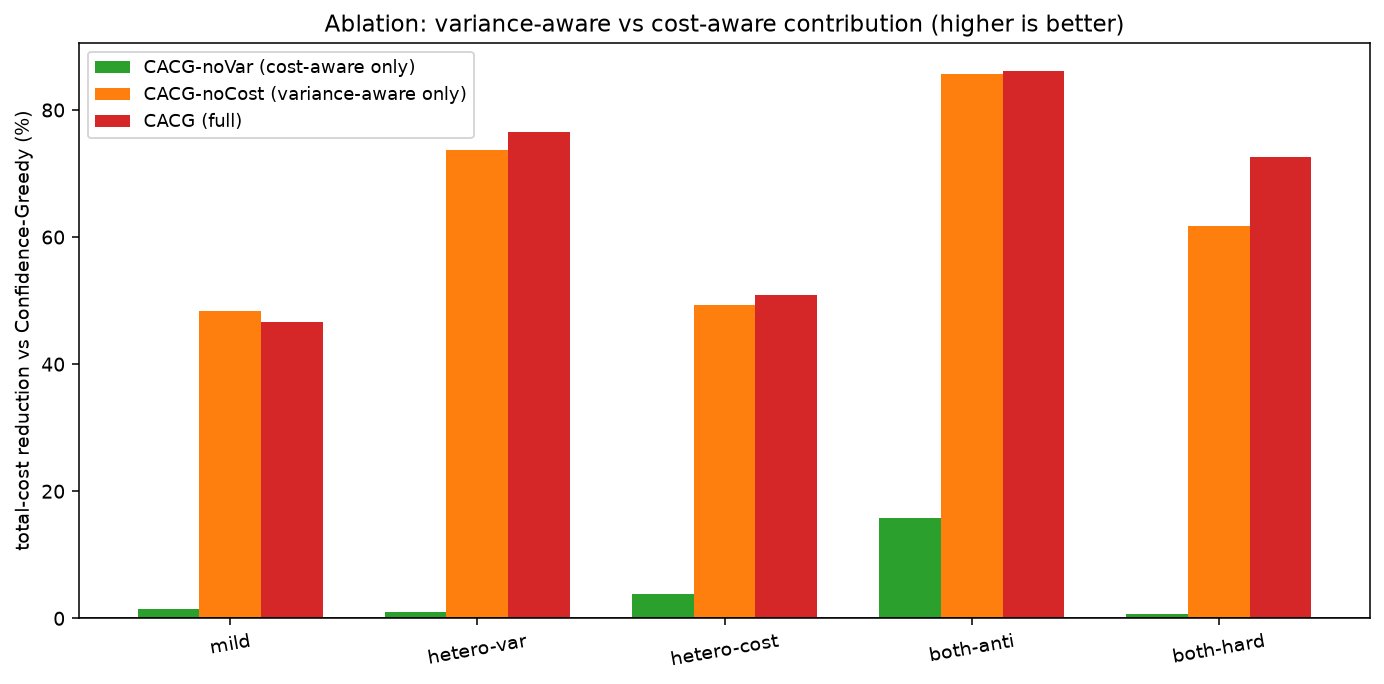
\includegraphics[width=0.78\textwidth]{figs/fig_vs_conf.png}
\caption{Ablation: total-cost reduction relative to \textsc{Conf-Greedy}.
Variance-adaptivity (\textsc{CACG-noCost}) is the dominant contributor;
cost-awareness adds on top in cost-dominated and hard regimes.}
\label{fig:ablation}
\end{figure}

\paragraph{Findings.}
(1) \emph{Adaptivity is the largest factor:} CACG cuts total cost by
$98$--$100\%$ versus the guaranteed non-adaptive baseline.
(2) \emph{Versus the certifying \textsc{Conf-Greedy}, CACG saves
$47$--$86\%$} at no loss of quality ($f(S)$ within $0.6$ of exact greedy).
(3) \emph{Attribution} (Fig.~\ref{fig:ablation}): variance-adaptivity
dominates; cost-awareness contributes in cost-heavy/hard regimes
(\texttt{both-hard}: $62\%\!\to\!73\%$ saved).
(4) The empirical-variance sub-Gaussian radius outperforms Maurer--Pontil,
whose range term dominates at small samples.
(5) \emph{Correctness:} empirical failure rate is $0.00$ in all regimes,
consistent with Theorem~\ref{thm:hp}.
(6) \emph{Anytime/certificate} (Fig.~\ref{fig:budget}): the budget--quality
curve is monotone and plateaus at greedy; certificate validity is
$\Pr[L\le f(S)]=0.976\ge 1-\delta=0.90$ (the guarantee holds, with margin).
(7) \emph{Robustness:} total cost varies only $\sim5\%$ across the
cost-exponent $p\in[1,2]$.

\begin{figure}[H]
\centering
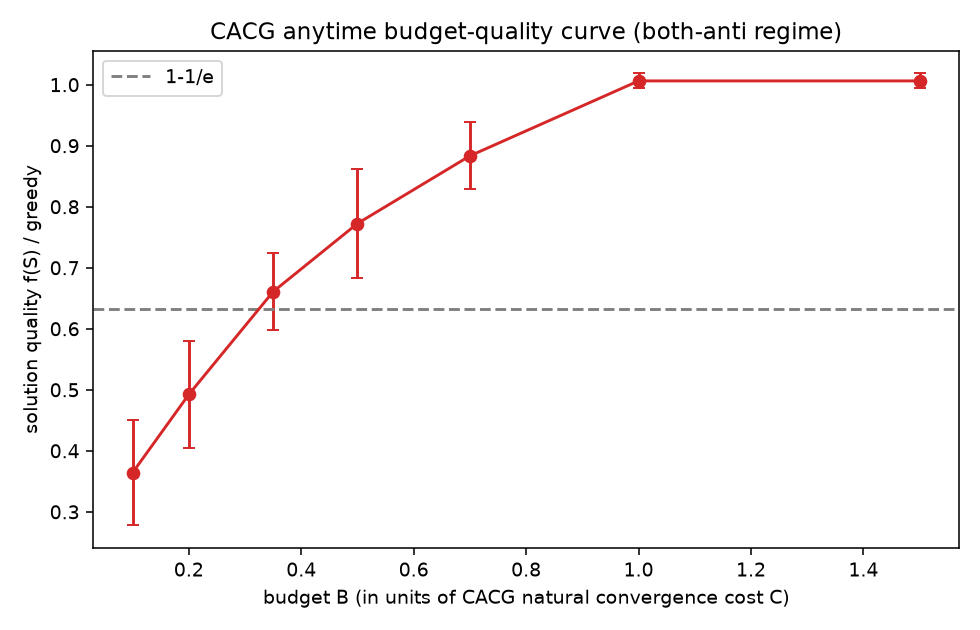
\includegraphics[width=0.62\textwidth]{figs/fig_budget_curve.png}
\caption{CACG anytime budget--quality curve (\texttt{both-anti}). Quality
rises monotonically with budget and saturates at greedy; the dashed line is
$1-1/e$.}
\label{fig:budget}
\end{figure}

% ====================================================================
\section{Related Work, Limitations, and Future Work}\label{sec:related}

\paragraph{Related work and honest positioning.}
CACG's ingredients each have precedent, which we cite to be transparent:
confidence/adaptive sampling to cut queries~\cite{Singla2016,ChenXingCrawford2023};
per-round BAI with a sampling allocation~\cite{ChenCrawford2024} (the
closest work); the square-root cost-aware rule from Cost-Aware
BAI~\cite{Kanarios2024}; empirical-variance
bounds~\cite{MaurerPontil2009,Audibert2009} and heterogeneous-variance
BAI~\cite{SHAdaVar2023}; and anytime lower-bound certificates as used in
online influence maximization~\cite{TangTangXiaoYuan2018}. What we can
\emph{honestly} claim is twofold: (i) a \emph{unifying survey lens}---these
methods are instances of one ``per-round approximately-maximal marginal $+$
sampling-budget allocation'' framework; and (ii) that, to the best of our
knowledge, \emph{optimizing total query cost under simultaneously
heteroscedastic and heterogeneous-cost queries inside the submodular greedy
loop has rarely been made explicit}. We deliberately avoid any ``first/novel
primitive'' claim.

\paragraph{Limitations and future work.}
Our guarantees assume benign re-sampleable noise and a direct marginal
oracle (Remark~\ref{rem:scope}). Extending to (a) persistent/adversarial
noise~\cite{HassidimSinger2017,Bhawalkar2025}; (b) the shared-baseline
correlation when only $f$ is queryable (e.g.\ influence maximization via
RR-sets~\cite{Borgs2014,TangShiXiao2015}); (c) matroid and non-monotone
constraints~\cite{CCPV2011,BuchbinderFNS2015}; (d) a rigorous cost
complexity for the cost-aware order and a matching cost lower bound; and
(e) fully unknown variances, are natural next steps.

\paragraph{Conclusion.}
We surveyed submodular maximization under noisy value queries through the
lens of the noise model, gave complete proofs of the classical and noisy
greedy guarantees, and contributed CACG, a cost-aware, variance-adaptive
confidence greedy with a high-probability $(1-1/e)\OPT-\varepsilon$
guarantee and an instance-dependent cost complexity. Experiments show large,
attributable savings in total query cost, with variance-adaptivity the
dominant driver---an honest, quantified account of a combination of known
techniques.

% ====================================================================
\bibliographystyle{plain}
\bibliography{references}

\end{document}
